\newpage
\section{Execution and Results} \label{sec:results}
    \subsection{Optimization of Settings}
    Before we started with the actual measurements, we optimized the settings.
    First of all, the parameter $\Delta m$, the resolution \texttt{res} and acceleration voltage $U$ had to be chosen optimally. Additionally, the two detector types Faraday and SEM were compared. The residual gas spectrum of the vacuum chamber was recorded for different settings. Since we assume that the residual gas consists primarily of air, we excluded atoms heavier than 50~amu and limited our scans to the range of 1 to 50 amu. For the step sizes we chose 0.2 amu and carried out 7 measurement runs. If nothing else is written, 70 V was selected as $U$.
    
    $\Delta m$ setting affects the offset of the line. To optimize $\Delta m$ we set \texttt{res} = 0\% and performed measurements for $\Delta m = -10\%, -5\%, 0\%, 5\%, 10\%, 15\%, 20\%, 35\%$.  The curves for $\Delta m = -10\%, 5\%, 20\%, 35\%$ are shown in the figures .... for the areas where they differ significantly from 0.
    
    When looking at these curves we notice that the larger $\Delta m$ gets, the less pressure is measured. So the sensitivity decreases strongly with increasing $\Delta m$. Additionally we can see
    that the smaller $\Delta m$ is chosen, the wider the curves become. In order to avoid an overlapping of the individual curves in case of neighboring mass peaks, $\Delta m$ must not be too large. We chose $\Delta m= 20\%$ as the optimal mixture of sensitivity and curve width. 
    
    The smaller the atomic mass, the stronger the sensitivity increases with decreasing $\Delta m$. This is especially visible in the range of amu = 1, where the peak with decreasing $\Delta m$ becomes larger than the peak in the range of amu = 2. This is in accordance with the descriptions of the parameter $\Delta m$ in the manual \cite{manual}. 
    
    To optimize \texttt{res}, which affects the slope of the work line, we chose $\Delta m = 20\%$ and varied \texttt{res} = -5\%, 5\%, 10\%. The results at the relevant ranges are shown in figures. 
    
    We find that \texttt{res} has hardly any influence on the sensitivity close to amu = 0, but a clearly discernible influence in the range of amu = 44. This fact was also described in the manual. Since \texttt{res} does not have a strong influence even in the larger range, we decided to set \texttt{res} in the later measurements neutral to 0\%. 
    
    To select the optimum $U$, $\Delta m = 20 \%$, \texttt{res} = 5\% was kept constant and the voltages of 50~V, 70~V and 90~V were tested. For most of the peaks the sensitivity was higher the lower the $U$ was (see). This may have to do with the fact that at low voltage less double ionization occurs. Therefore we decided to use an $U$ of 50~V.  
    
    Finally we now come to compare the two detectors. For this purpose, both detectors were measured with \texttt{res} = 5\%, $\Delta m = 20\%$ and $U$ = 70~V. As we can see from the figure ..., the sensitivity of the Faraday detector is significantly higher than that of the SEM. Therefore we decided to use the Faraday detector for our measurements. 
    
    In summary, the parameters are optimal if $\Delta m = 20\%$, \texttt{res} = 0\%, $U$ = 50~V and the faraday detector is selected. 
    
    \subsection{Residual gas Identification}
    \subsection{Noble Gas Analysis}
    \begin{figure}[h!]
    \centering
    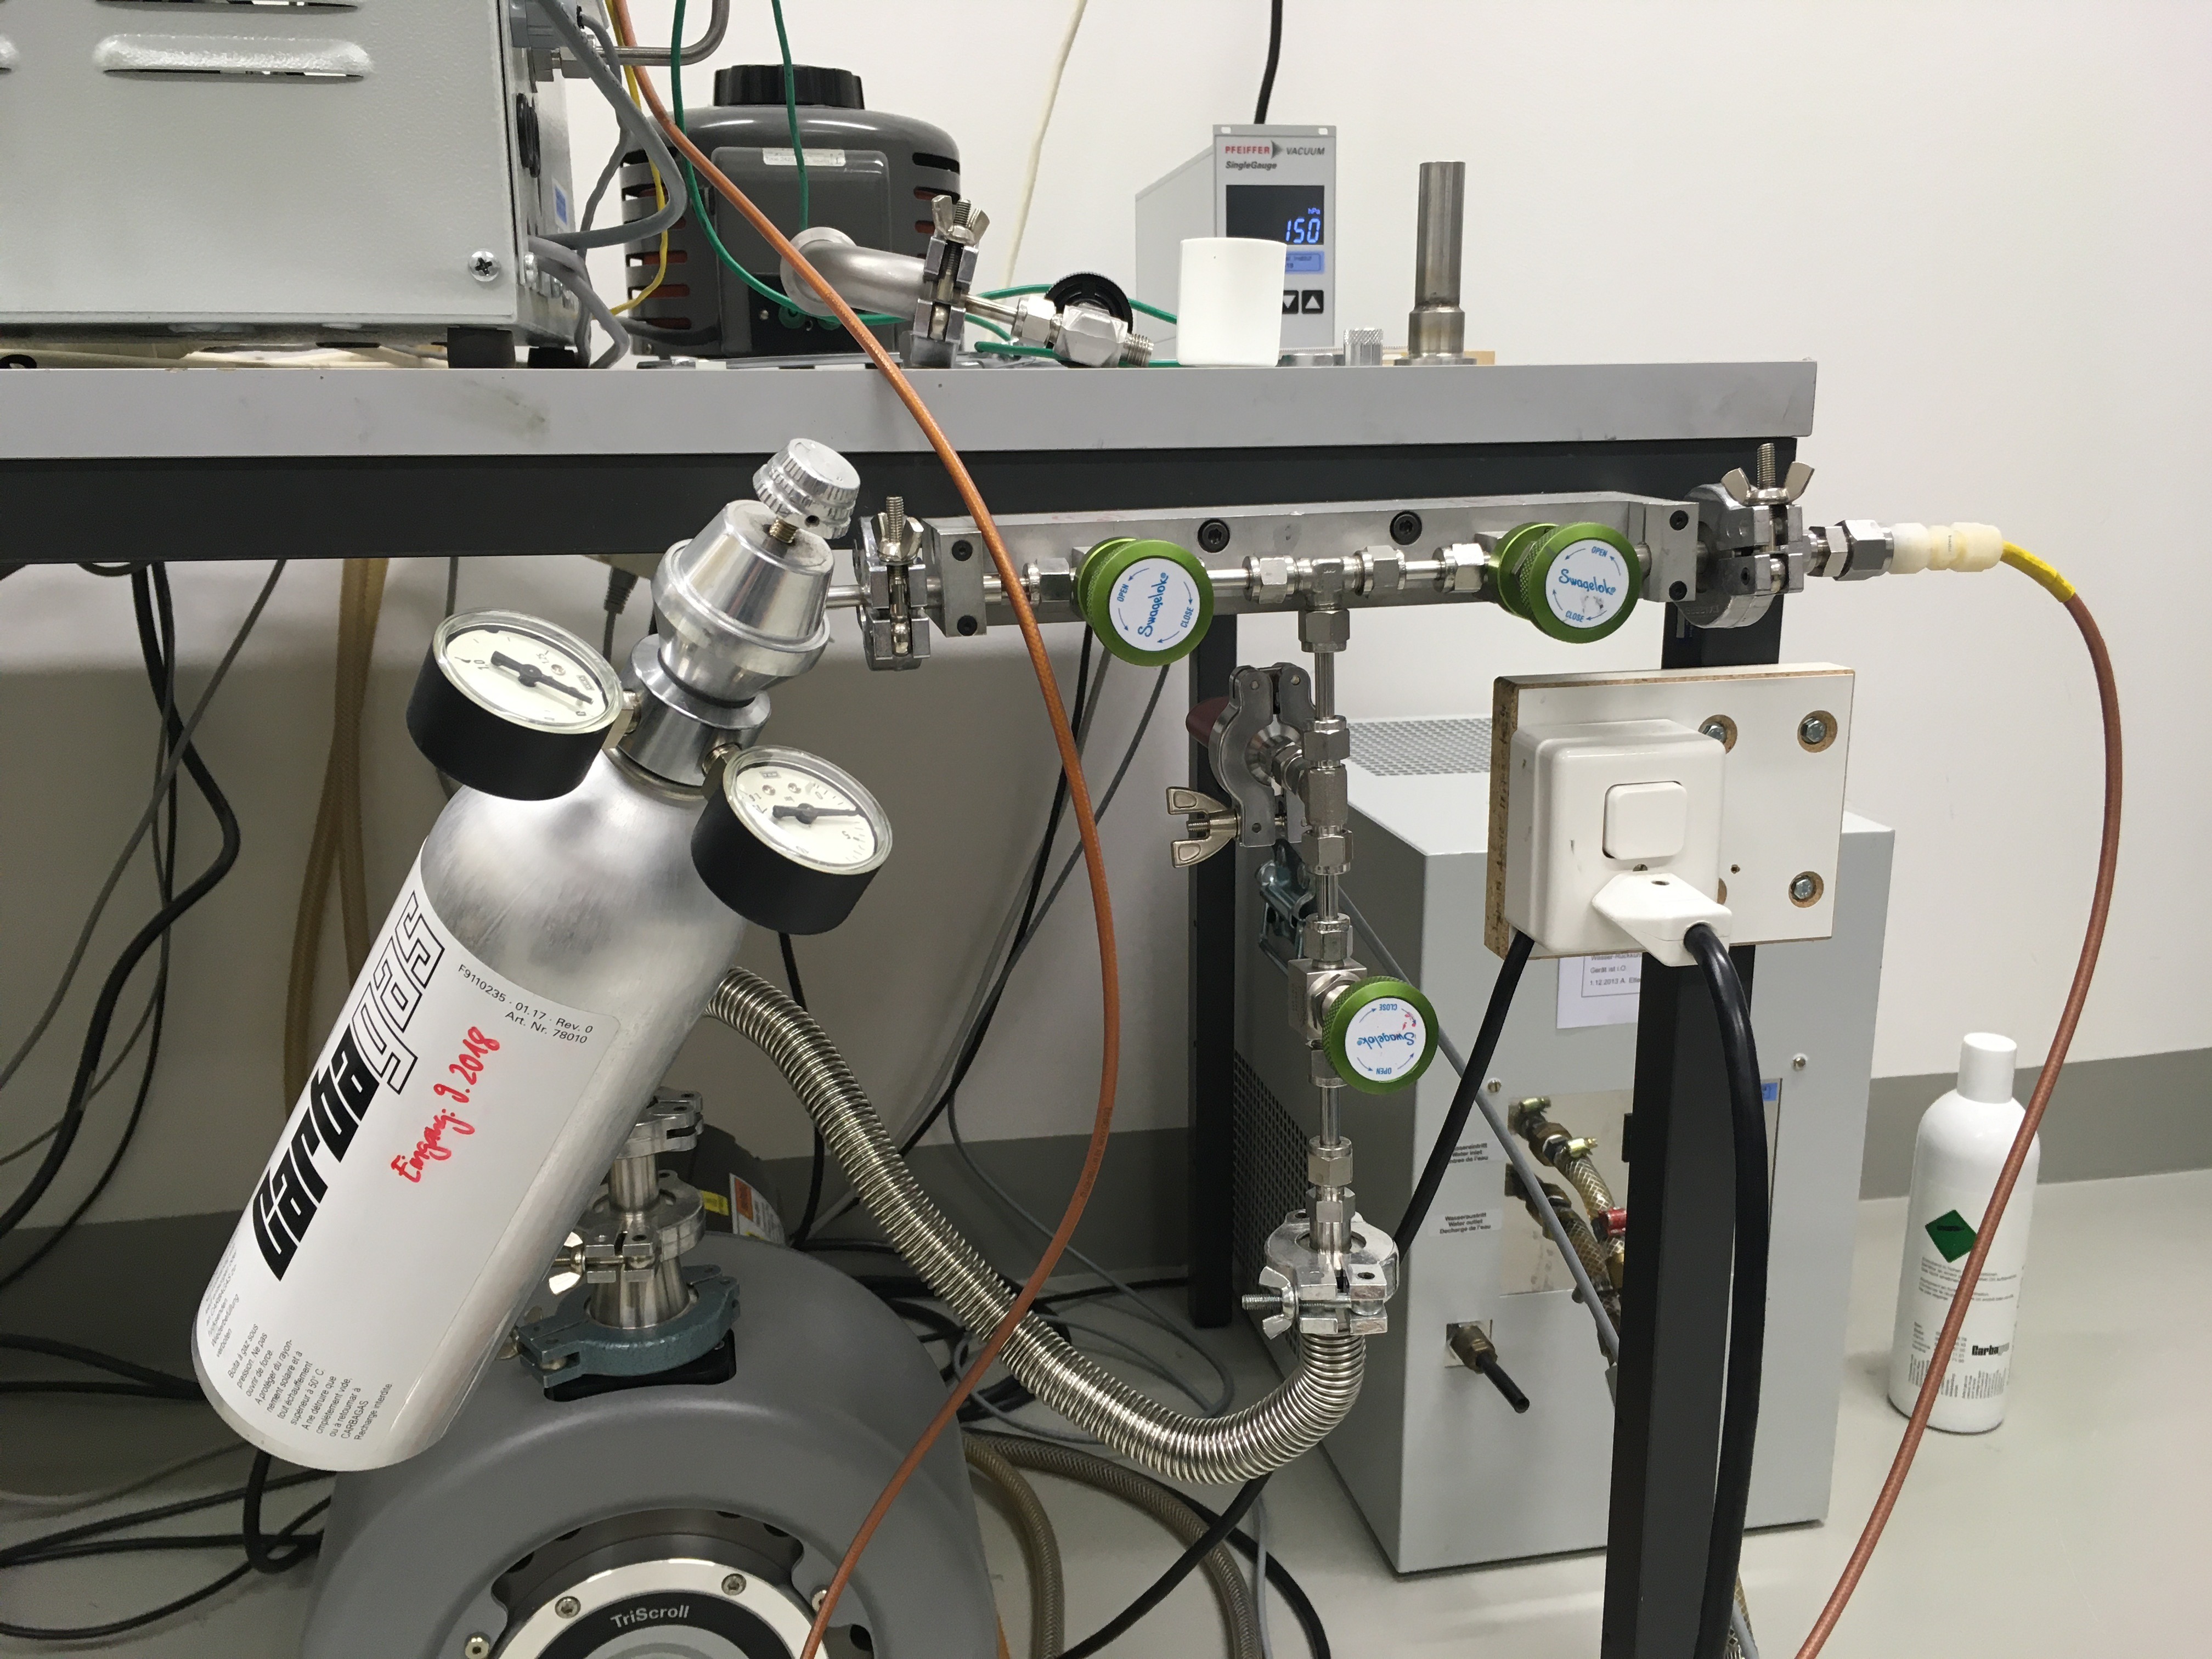
\includegraphics[width=0.5\textwidth]{Report/pictures/cartridge.JPG}
    \caption{The setup with an attached noble gas cartridge.}
    \label{fig:noblegas}
    \end{figure}
    
    \subsection{Inhaled Air}
    \begin{figure}
        \centering
        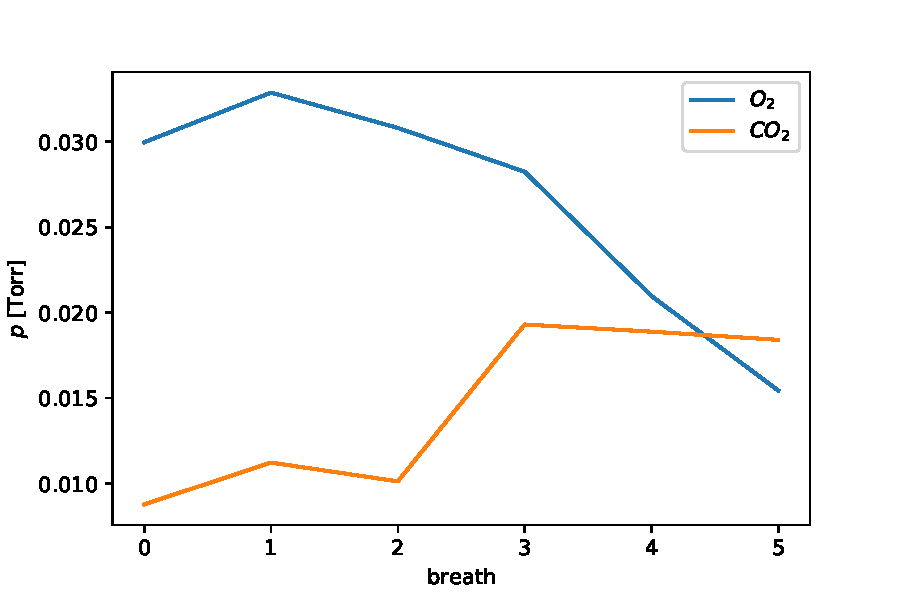
\includegraphics[width=\textwidth]{Report/DataResultsPlots/air.pdf}
        \caption{CO$_2$ and O$_2$ amount in Inhaled air.}
        \label{fig:air}
    \end{figure}
    
    
    
    \subsection{Measurement of Ethanol}
    
    \begin{figure}[h!]
    \centering
    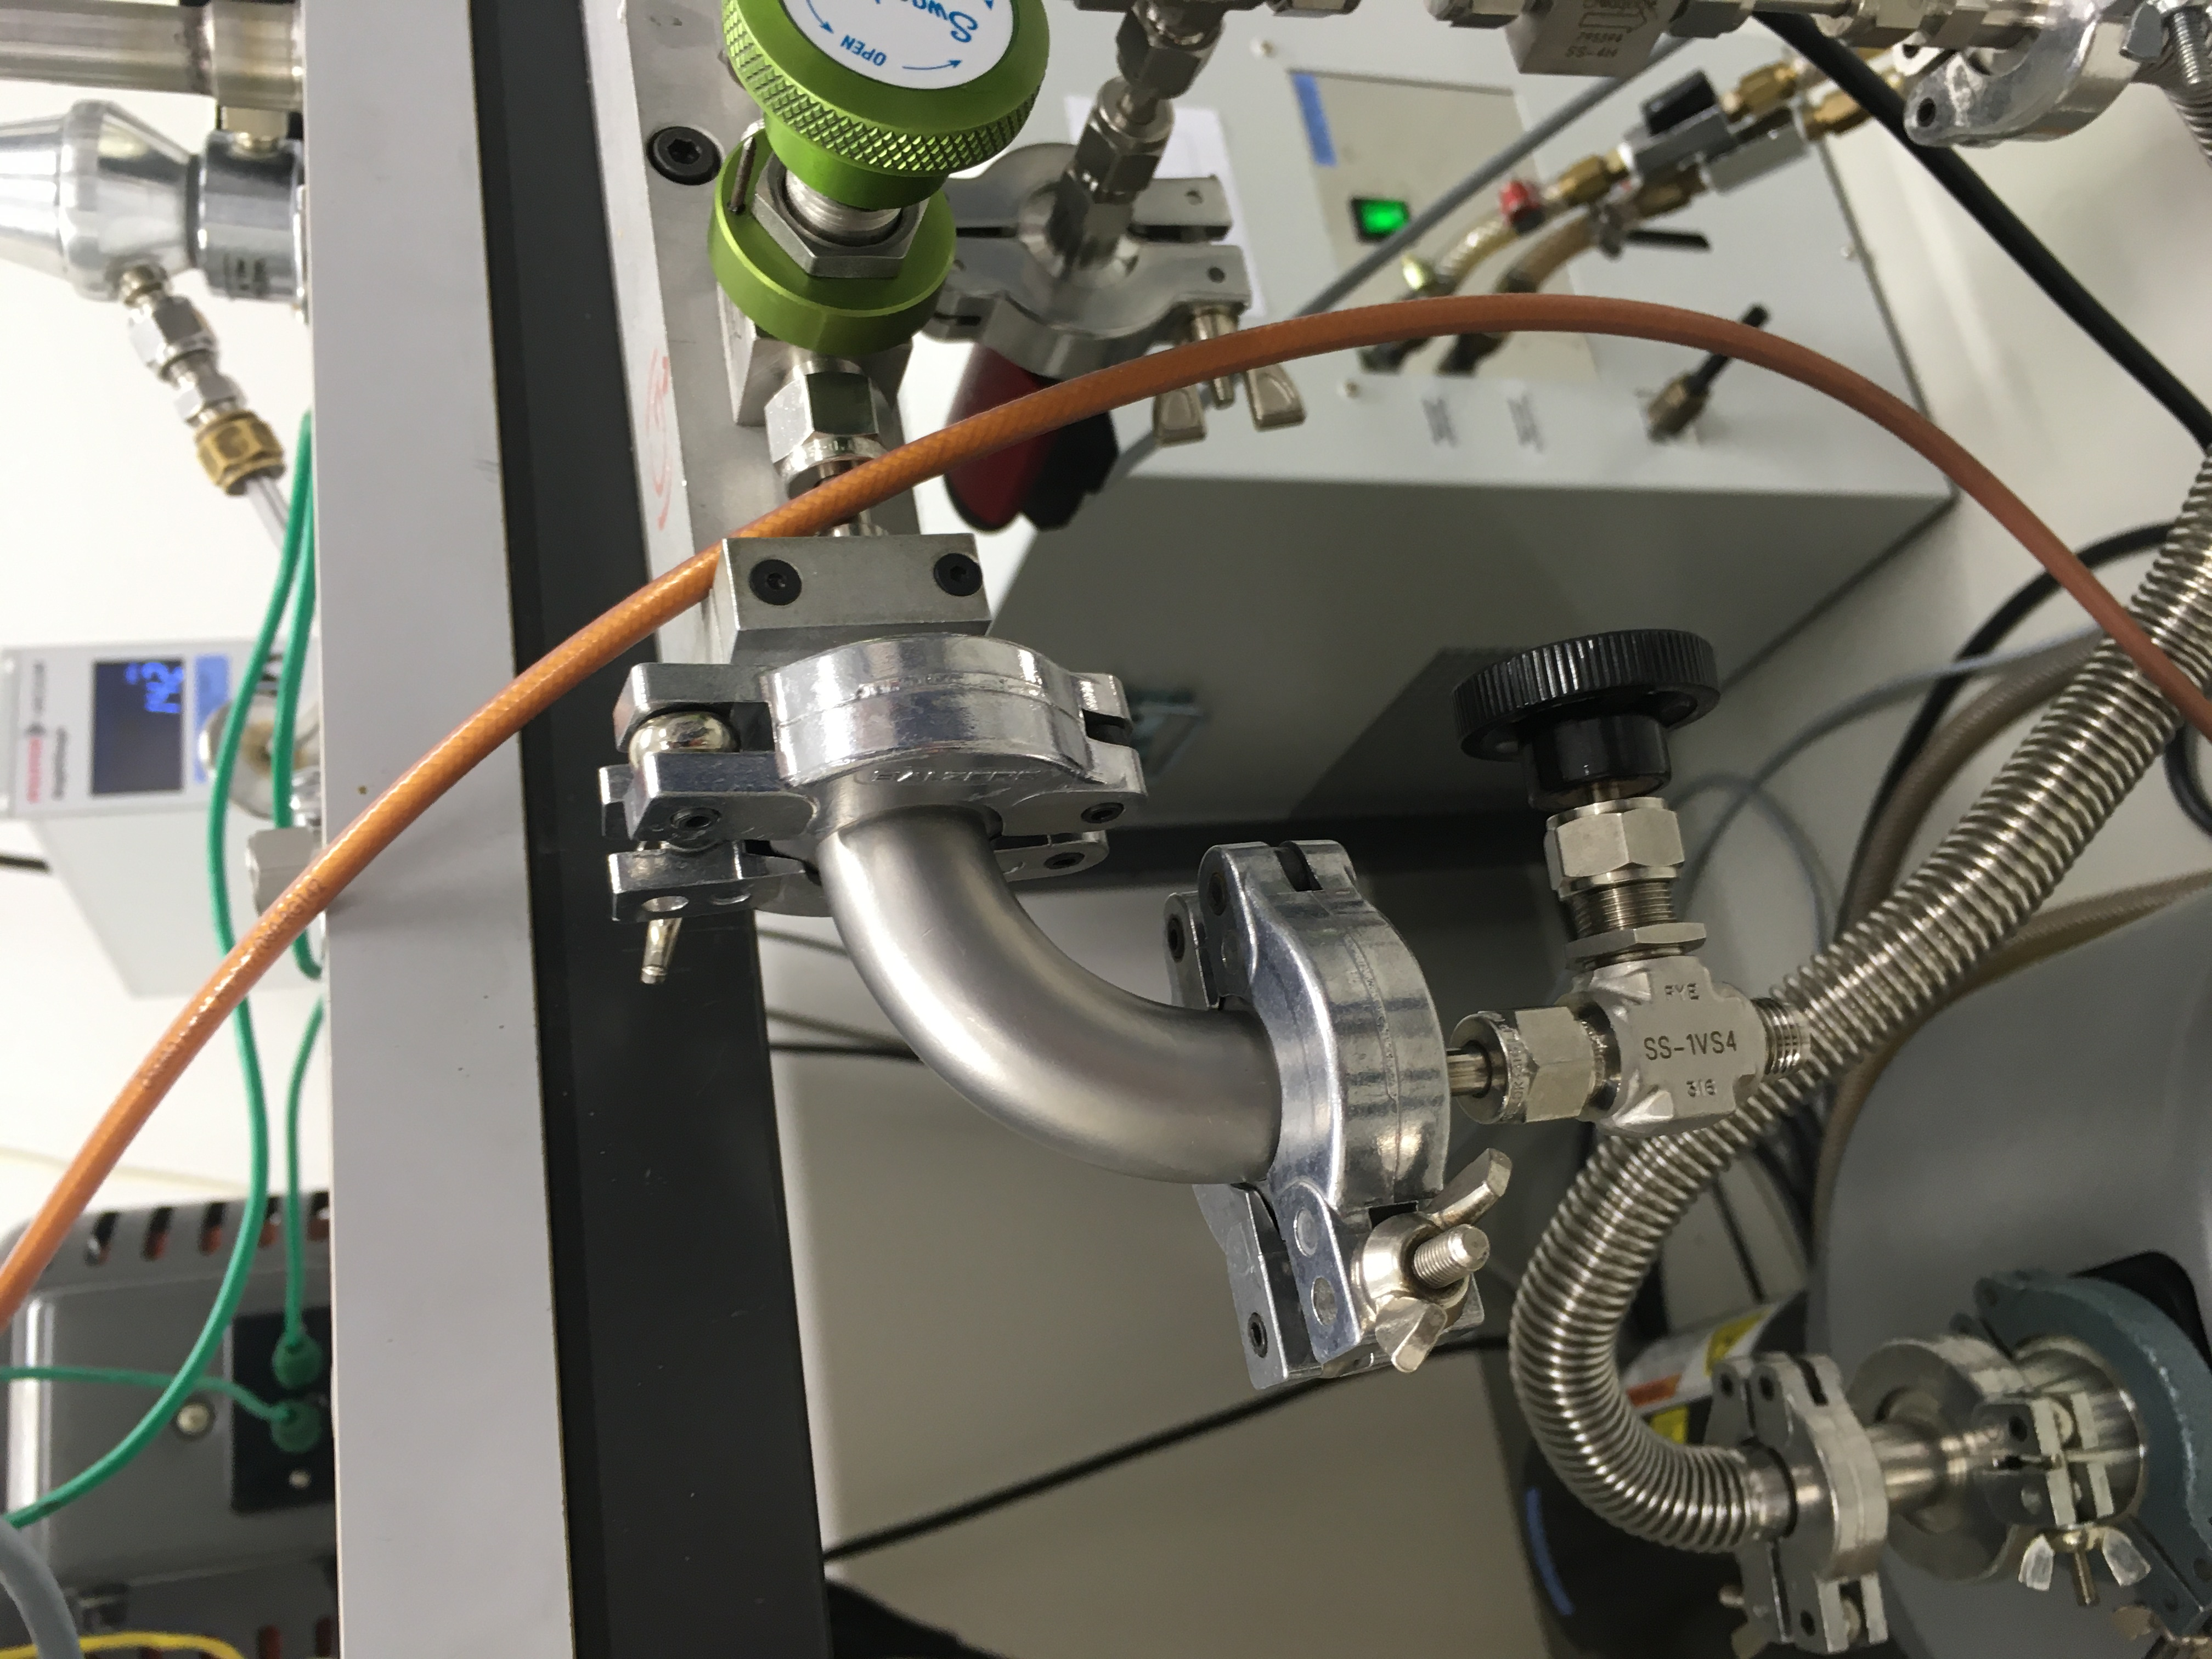
\includegraphics[angle=-90, origin=c, width=0.5\textwidth]{Report/pictures/liquids.JPG}
    \caption{The setup to attach a liquid sample to the system. The gaseous phase will be pumped to the mass spectrometer while the liquid phase will stay inside the container.}
    \label{fig:ethanol}
    \end{figure}
    
    \subsection{Deo and Sparkling Water Analysis}
    
    \begin{figure}[h]
            \centering
            \subfloat[balloon with CO2 from sparkling water]{\label{figure:sparkling}
                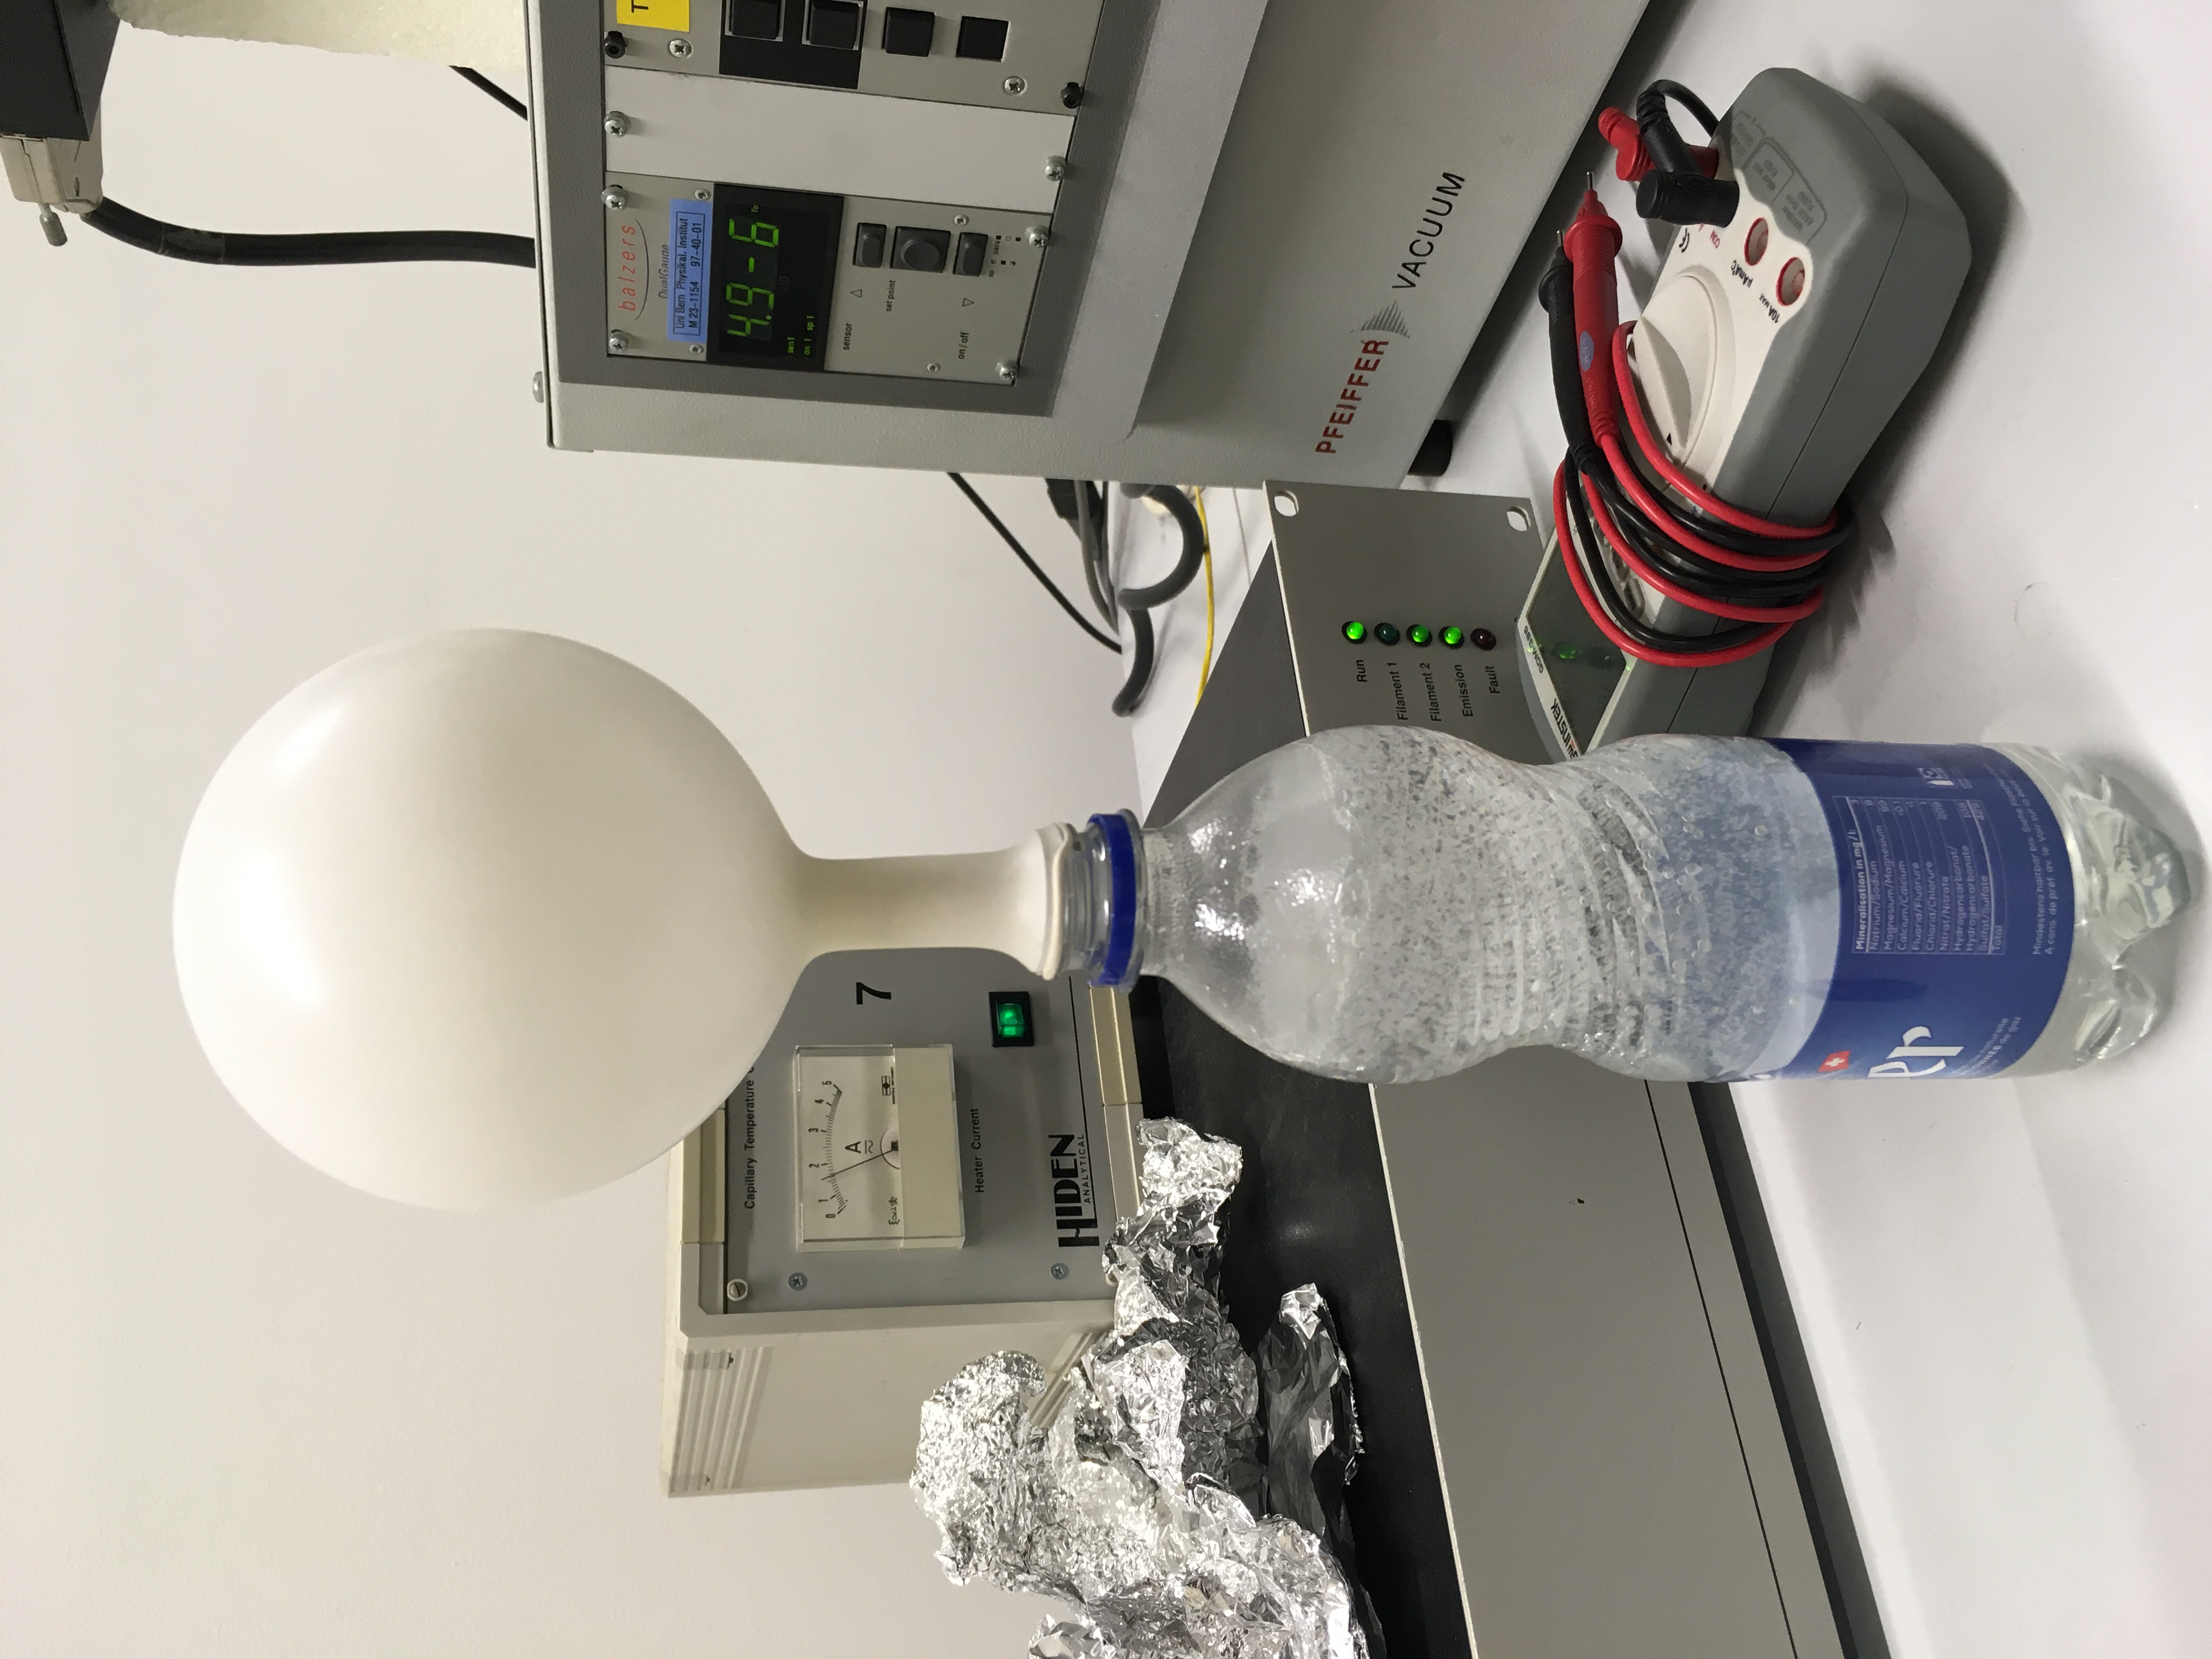
\includegraphics[width=0.47\textwidth, angle=270, origin=c]{Report/pictures/ballon_bottle2.JPG}}\quad
            \subfloat[balloon attached to the system]{\label{figuer:sparkling2}
                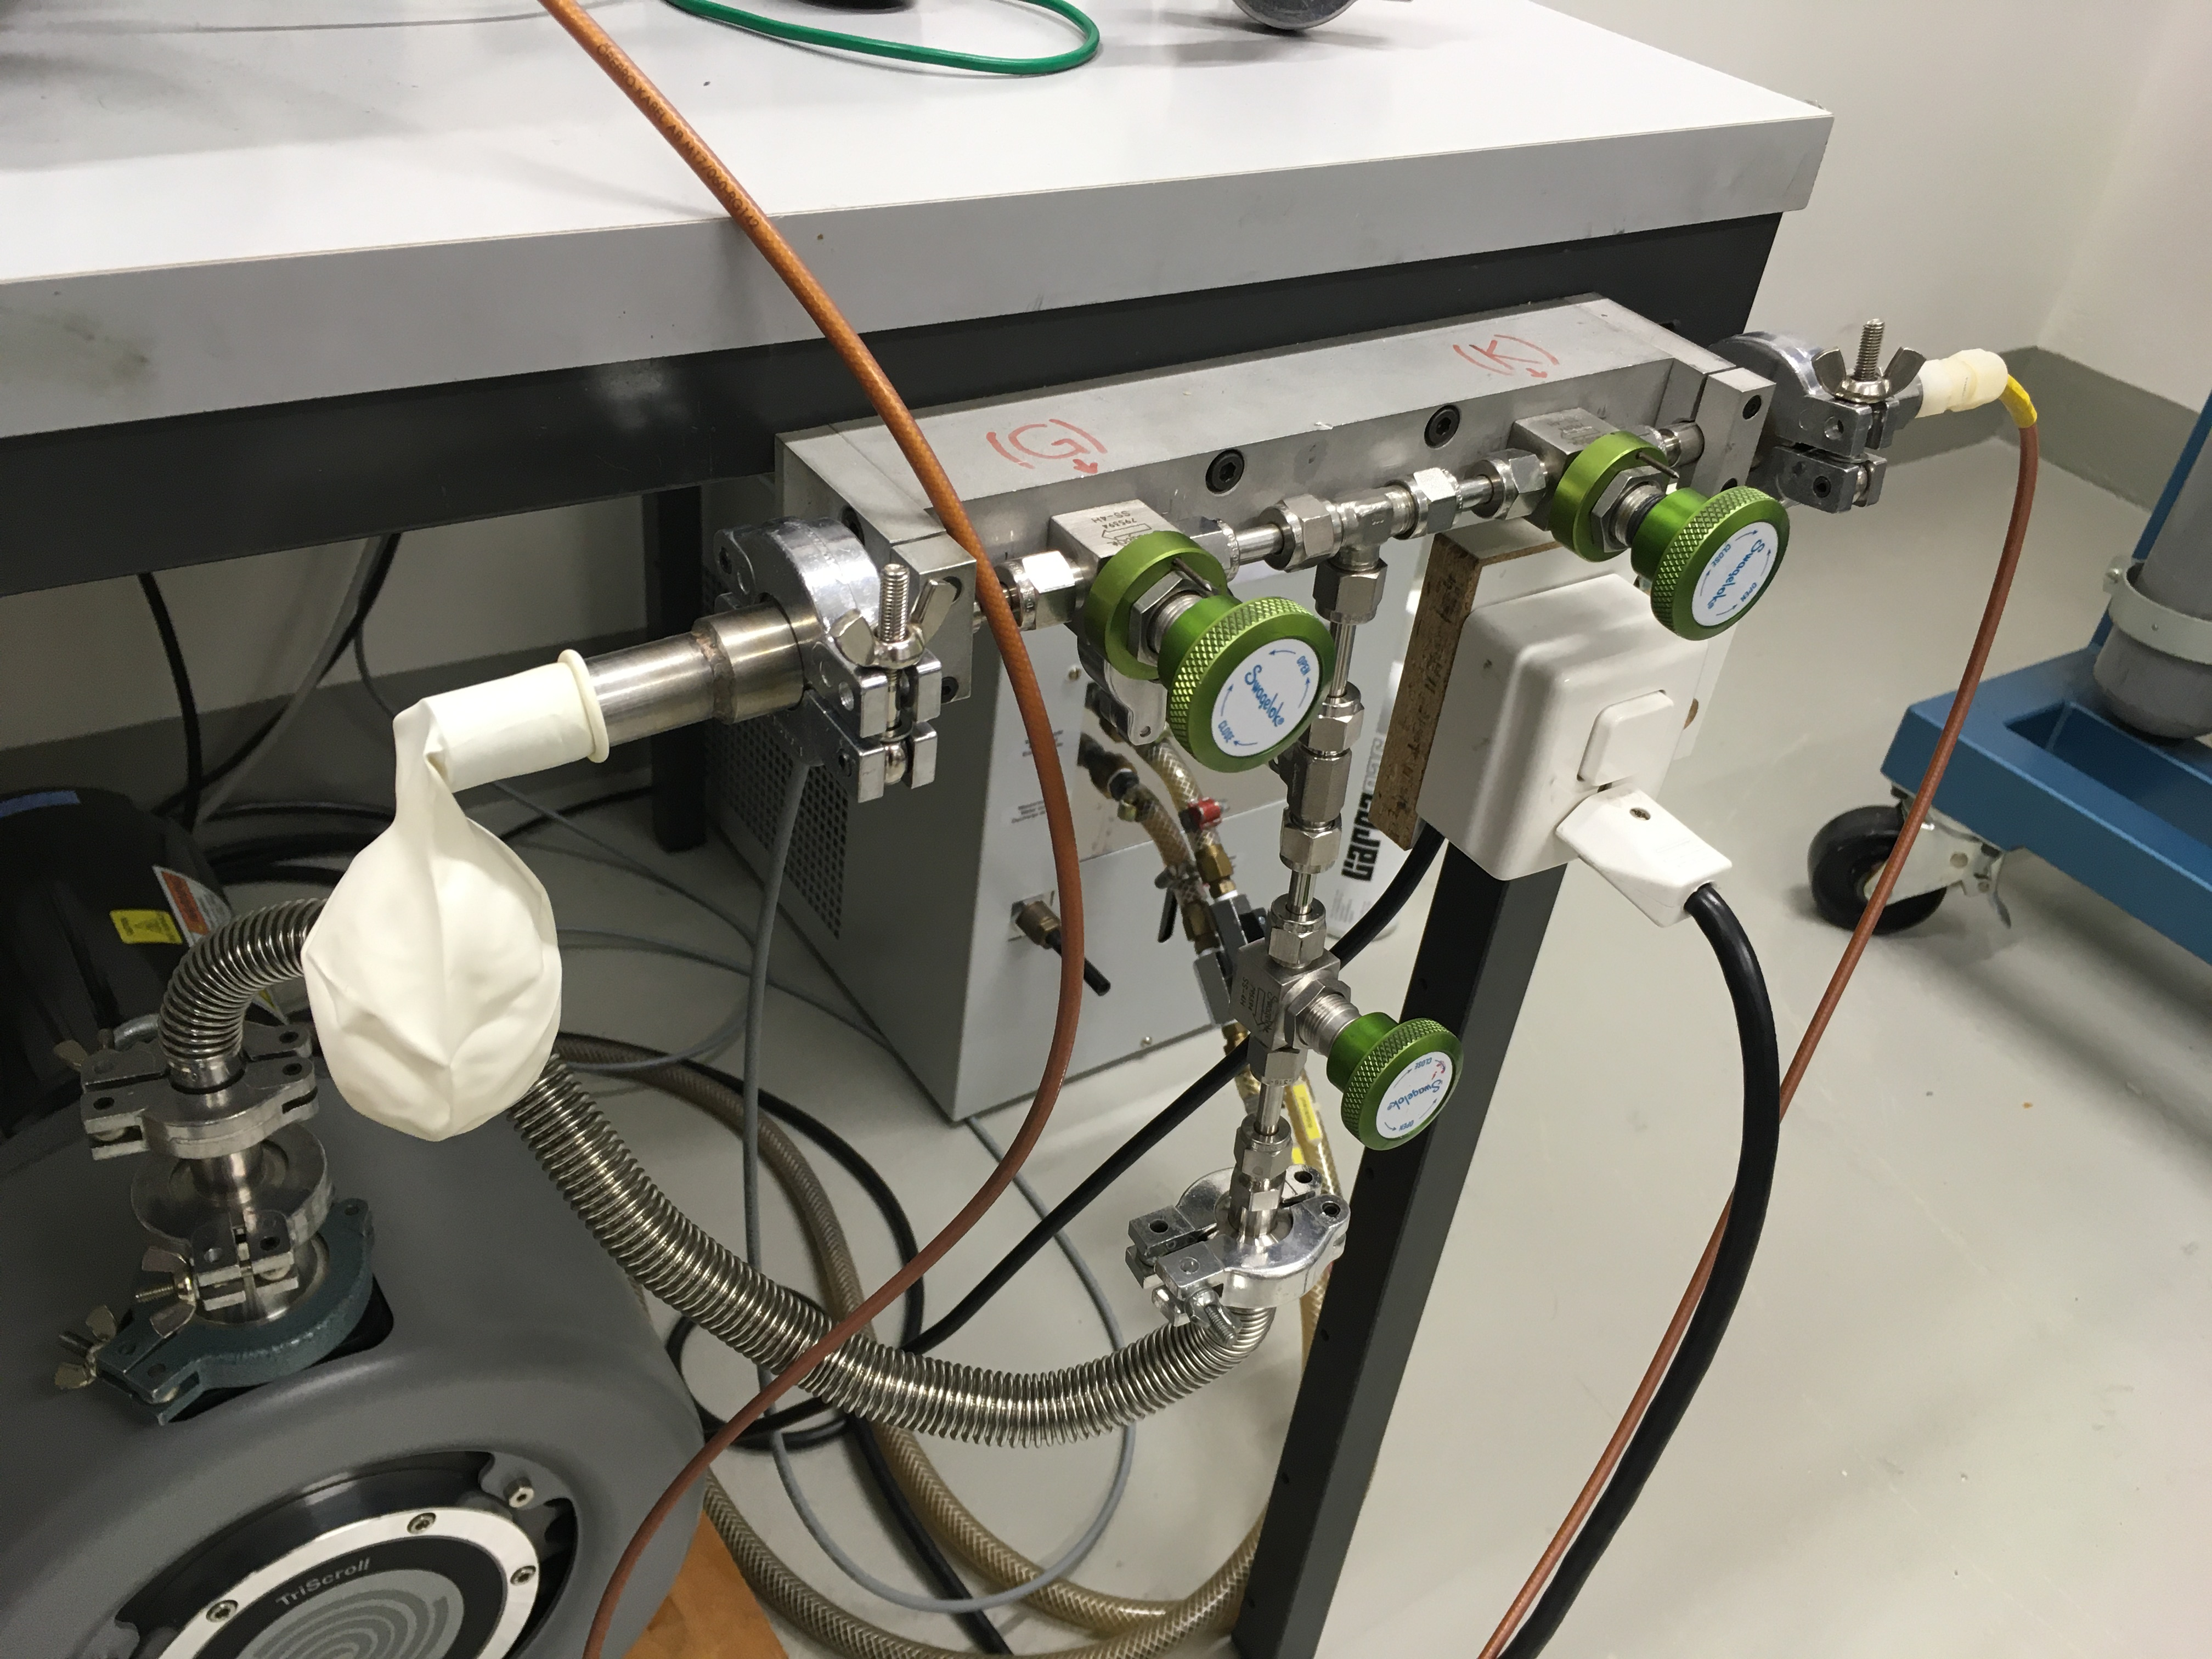
\includegraphics[width=0.47\textwidth]{Report/pictures/ballon_setup.JPG}}\quad
            \caption{The setup of the experiment with samples filled into a balloon.}
            \label{fig:setup2}
    \end{figure}